\section{Supplementary material}
\subsection{Data sets and metadata}
In figure \ref{fig:selection} we summarize the literature selection process that produced our sample. Table \ref{tab:metadata} shows the main metadata referring to the datasets included in the analysis. Those for which the Code of Paper includes the string \texttt{cchunts} are published in the \texttt{R} package with the same name, associated to the paper from \citet{koster_life_2020}. These were compiled by Koster, who ``searched for relevant studies on subsistence hunting in the anthropological and biological literature, subsequently contacting authors to invite them to contribute data. The contributors submitted data in a standardized format that included variables for the biomass acquired on terrestrial hunting trips, the ages of the hunters at the time of the hunt, the duration of the trip, the hunting weaponry carried by the hunters, and the presence of dogs or assistants" \citep{koster_life_2020}.

Following inclusion of data from this source, we screened the data we extracted from published papers to remove repeated data sets. In particular, data relative to the Ache of Paraguay extracted from \citet{walker_age-dependency_2002} have not been used because they are already present in the "Hill\_Kintigh" data set included in the \texttt{cchunts} package. 

Tsimane data extracted from \citet{gurven_how_2006} are a repetition of those included in the \texttt{cchunts} data (``Trumble\_Gurven"). Only the latter were used in the analysis.

%Pume' foraging data presented in \cite{kramer_early_2009} refer to underground storage resources, whereas Pume' data in the \texttt{cchunts} package are hunting returns, hence both data have been included in the analysis.

Data collected by Bliege Bird and Bird among the Martu in Western Australia come from both a 2005 study on children foraging \citep{bird_mardu_2005} and from the dataset in the \texttt{cchunts} package \citep{koster_life_2020}. The 2005 paper reports data from individual of both sexes between 5 and 14 years old hunting goanna lizards in the rocky outcrop not far from the camp. These data were collected by the authors between 2000 and 2002. The \texttt{cchunts} data were collected between 2002 and 2010, are relative to individuals aged 7 to 79 and partially exclude female contributions (``This data set includes observations of female foragers when they were accompanied by men on trips, but not women on foraging trips that did not include male foragers"). The two data set are thus not fully overlapping, but there is the possibility that some data are present in both sets. In particular, 14 foraging returns collected in 2002 from individuals below 14 years old are present in the \texttt{cchunts} data set and could hence have been included in \citet{bird_mardu_2005}. Looking in detail at these subsets, they do not appear to be repetitious (a 9 years old boy present in the \texttt{cchunts} dataset does not appear in the \citet{bird_mardu_2005} study, for example, and none of the younger individuals' returns reported here appear in \texttt{cchunts}). 

\begin{figure}[h]
\renewcommand{\thefigure}{S\arabic{figure}}
\setcounter{figure}{0}
    \begin{tikzpicture}[node distance=2cm]
        \node (SD) [rec] {Science Direct: 25};
        \node (JS) [rec, right=0.1 of SD] {JStor: 59};
        \node (GS) [rec, right=0.1 of JS] {Google Scholar: 320};
        \node (PN) [rec, right=0.1 of GS] {PsycNet: 0};
        \node (SP) [rec, right=0.1 of PN] {Springer: 75};
        \node (WI) [rec, right=0.1 of SP] {Wiley: 23};
        \node (AD) [mainrec, below=1.5 of GS] {After removing duplicates: 360};
        \node (AF) [mainrec, below=0.8 of AD] {After full text checked: 35};
        \node (IO) [mainrec, right=2 of AF] {Included from bibliographies and CVs: 5};
        \node (MA) [mainrec, below right=0.8 and -1 of AF] {Meta-data investigated: 40};
        \node (SS) [mainrec, below =0.8  of MA] {Selected papers: 13};
        \node (IA) [mainrec, below =0.8  of SS] {Included in analysis: 38}; %\Sexpr{nlevels(unique(d[,"study"]))}
        \node (CC) [mainrec, below left =0.8  and 0.3 of MA] {From \texttt{cchunts} package: 26}; %\Sexpr{nlevels(unique(d[,"study"])) - 12}
        \node (GW) [rec, right=0.3 of SS] {Excluded as duplicated in the \texttt{cchunts} package: 2};
        \draw[->,line width=1] (SD) -- (AD);
        \draw[->,line width=1] (JS) -- (AD);
        \draw[->,line width=1] (GS) -- (AD);
        \draw[->,line width=1] (PN) -- (AD);
        \draw[->,line width=1] (SP) -- (AD);
        \draw[->,line width=1] (WI) -- (AD);
        \draw[->,line width=1] (AD) -- (AF);
        \draw[->,line width=1] (AF) -- (IO);
        \draw[->,line width=1] (AF) -- (MA);
        \draw[->,line width=1] (IO) -- (MA);
        \draw[->,line width=1] (MA) -- (SS);
        \draw[->,line width=1] (SS) -- (IA);
        \draw[->,line width=1] (CC) -- (IA);
        \draw[->,line width=1] (SS) -- (GW);
    \end{tikzpicture}
    \caption{\textbf{Process of paper selection.}}
    \label{fig:selection}
\end{figure}



% Please add the following required packages to your document preamble:
% \usepackage[table,xcdraw]{xcolor}
% If you use beamer only pass "xcolor=table" option, i.e. \documentclass[xcolor=table]{beamer}
% \usepackage{lscape}
% \usepackage{longtable}
% Note: It may be necessary to compile the document several times to get a multi-page table to line up properly
\begin{landscape}
\begin{longtable}{M{2.6cm} M{3.6cm} M{1.5cm} c c M{1cm} c c}
\caption{\textbf{Metadata for included datasets.} These are relative to each source of foraging returns data included in the analysis. The first 11 datasets have been extracted from published papers, the remaining were part of the \texttt{cchunts} package. As sample size we report the total number of observations for foraging returns, with the total number of foragers under 20 years included in our analysis in parentheses. }\\
\hline
\rowcolor[HTML]{C0C0C0} 
Code of data                  & Paper                                     & Population      & Years      & Unit      & Resource           & Ages    & Sample size \\ \hline
\endfirsthead
%
\endhead
%
\rowcolor[HTML]{EFEFEF} 
Bird\_2005                     & \cite{bird_mardu_2005}                    & Martu           & 2000-2002  & kcal/hr   & game               & 4- 14   & 157 (22)    \\
BliegeBird\_1995               & \cite{bird_children_1995}                 & Meriam          & 1993       & g/min     & fish, fruit, mixed & 3-14    & 12(12)      \\
\rowcolor[HTML]{EFEFEF} 
BliegeBird\_2002a              & \cite{bird_constraints_2002}              & Meriam          & 1993-1998  & kcal/hr   & fish               & 4-75    & 196(42)     \\
BlurtonJones\_1989             & \cite{blurton_jones_modelling_1989}       & Hadza           & 1985-1986  & g/hr      & USO, mixed, fruit  & 2- 20+  & 70 (29)     \\
\rowcolor[HTML]{EFEFEF} 
BlurtonJones\_1997             & \cite{blurton_jones_why_1997}             & Hadza           & 1986- 1989 & kcal/hr   & USO, fruits        & 2-18    & 61 (61)     \\
BlurtonJones\_2002             & \cite{blurton_jones_selection_2002}       & Hadza           & 1997       & kg/hr     & USO                & 6-75    & 79 (46)     \\
\rowcolor[HTML]{EFEFEF} 
Bock\_2005                     & \cite{bock_what_2005}                     & Bugakwhe, etc & 1994       & kcal/hr   & fish               & 5- 14   & 16 (16)     \\
Crittenden\_2013               & \cite{crittenden_juvenile_2013}           & Hadza           & 2005       & kcal/day & mixed              & 3-17    & 34 (34)     \\
\rowcolor[HTML]{EFEFEF} 
Froehle\_2018                  & \cite{froehle_physical_2019}              & Hadza           & 2005       & kcal/trip & mixed              & 5- 14   & 9 (9)       \\
Hawkes\_1995                   & \cite{hawkes_hadza_1995}                  & Hadza           & 1988       & g/hr      & USO, fruits        & 3-17    & 20 (17)     \\
\rowcolor[HTML]{EFEFEF} 
Tucker\_2005                   & \cite{tucker_growing_2005}                & Mikea           & 1997- 2003 & kcal/hr   & USO                & NA      & 254(37)     \\
Alvard\_cchunts                & \cite{alvard_shotguns_1995}               & Piro            & 1989-1991  & kg/trip   & game               & 15-70   & 42(5)     \\
\rowcolor[HTML]{EFEFEF} 
Beckerman\_cchunts             & \cite{beckerman_ecology_2013}             & Bari            & 1970-1972  & kg/trip   & game               & 12-55   & 18(9)    \\
Bird\_Bird\_Codding\_ cchunts     & \cite{bird_pursuit_2009}                  & Martu           & 2000-2010  & kg/trip   & game               & 7-79    & 77(21)     \\
\rowcolor[HTML]{EFEFEF} 
Coad\_cchunts                  & \cite{coad_bushmeat_2008}                 & Pouvi, etc    & 2004-2010  & kg/trip   & game               & 15- 69  & 70(7)     \\
Duda\_cchunts                  & \cite{reyes-garcia_adaptive_2016}         & Baka            & 2012-2013  & kg/trip   & game               & 16- 69  & 57(6)      \\
\rowcolor[HTML]{EFEFEF} 
Ellen\_cchunts                 & \cite{ellen_individual_1996}              & Nuaulu          & 1970       & kg/trip   & game               & 10-70   & 37(8)     \\
Fernandez\_Llamazares\_ cchunts  & \cite{reyes-garcia_adaptive_2016}         & Tsimane         & 2012-2013  & kg/trip   & game               & 15-70   & 29(4)     \\
\rowcolor[HTML]{EFEFEF} 
Franzen\_cchunts               & \cite{franzen_evaluating_2006}            & Waorani         & 2002       & kg/trip   & game               & 16- 77  & 48(4)      \\
Gallois\_cchunts               & \cite{reyes-garcia_adaptive_2016}         & Baka            & 2012-2013  & kg/trip   & game               & 16- 75  & 80(9)     \\
\rowcolor[HTML]{EFEFEF} 
Gueze\_cchunts                 & \cite{reyes-garcia_adaptive_2016}         & Punan           & 2012-2013  & kg/trip   & game               & 16- 61  & 35(2)      \\
Headland\_cchunts              & \cite{headland_why_1986}                  & Agta            & 1962-1984  & kg/trip   & game               & 13- 66  & 44(7)     \\
\rowcolor[HTML]{EFEFEF} 
Healey\_Nen\_PNG\_cchunts        & Preliminary fieldwork                     & Nen             & 2013       & kg/trip   & game               & 18- 46  & 7(2)        \\
Hill\_Kintigh\_ cchunts          & \cite{hill_can_2009}                      & Ache            & 1980-2007  & kg/trip   & game               & 11- 75  & 147(37)  \\
\rowcolor[HTML]{EFEFEF} 
Koster\_cchunts                & \cite{koster_hunting_2008}                & Mayanga         & 2004-2013  & kg/trip   & game               & 8- 63   & 52(17)     \\
Kramer\_Greaves\_cchunts        & \cite{kramer_why_2017}                    & Pume'           & 1990-2006  & kg/trip   & game               & 11- 65  & 23(9)     \\
\rowcolor[HTML]{EFEFEF} 
Lupo\_Schmitt\_cchunts          & \cite{lupo_upper_2002}                    & Bofi, Aka       & 1999-2002  & kg/trip   & game               & 6- 60   & 59(20)    \\
Pacheco\_cchunts               & \cite{pacheco-cobos_economic_2015}        & Maya            & 2011-2012  & kg/trip   & game               & 16- 60  & 59(10)     \\
\rowcolor[HTML]{EFEFEF} 
Pangau\_Adam\_cchunts           & \cite{pangau-adam_wildmeat_2012}          & Nimboran        & 2005-2006  & kg/trip   & game               & 16- 67  & 26(1)      \\
Ready\_cchunts                 & \cite{ready_food_2016}                    & Inuit           & 2013-2014  & kg/trip   & game               & 12- 55  & 15(4)       \\
\rowcolor[HTML]{EFEFEF} 
Reyes\_Garcia\_cchunts          & \cite{reyes-garcia_adaptive_2016}         & Tsimane         & 2012-2013  & kg/trip   & game               & 16- 91  & 37(2)      \\
Sillitoe\_cchunts              & \cite{sillitoe_managing_2004}             & Wola            & 1977       & kg/trip   & game               & 10- 45  & 27(10)    \\
\rowcolor[HTML]{EFEFEF} 
Siren\_cchunts                 & \cite{siren_effects_2016}                 & Quichua         & 1999, 2008 & kg/trip   & game               & 19- 59  & 32(1)      \\
Trumble\_Gurven\_cchunts        & \cite{gurven_how_2006}                    & Tsimane         & 2002-2011  & kg/trip   & game               & 7- 82   & 172(53)    \\
\rowcolor[HTML]{EFEFEF} 
Van\_Vliet\_ et\_al\_ Gabon\_cchunts & \cite{van_vliet_hunting_2008}             & Ba-Kota et al   & 2006-2007  & kg/trip   & game               & 15- 45  & 19(3)      \\
Venkataraman\_et\_al\_cchunts    & \cite{endicott_hunting_1979}              & Batek           & 1975-1976  & kg/trip   & game               & 9- 50   & 27(11)     \\
\rowcolor[HTML]{EFEFEF} 
Winterhalder\_cchunts          & \cite{winterhalder_boreal_1983}           & Cree            & 1975       & kg/trip   & game               & 15- 59  & 16(4)     \\
Yu\_et\_al\_cchunts              & \cite{ohl-schacherer_sustainability_2007} & Matsigenka      & 2004-2007  & kg/trip   & game               & 8- 52   & 69(18)   \\
\rowcolor[HTML]{EFEFEF} 
Ziker\_cchunts                 & \cite{ziker_peoples_2002}                 & Dolgan          & 1993-1997 & kg/trip   & game               & 15-66  & 26(3)     \\ 
\renewcommand{\tablename}{Table S}
\label{tab:metadata}
\end{longtable}
\end{landscape}


\subsubsection{Excluded datasets} \label{SI:excluded}

Several papers that passed the first rounds of selection (i.e. appeared to report original data on children foraging returns) were not included in the analysis for a variety of reasons. 

Some were subsequently found not to report relevant data \citep{blurton_jones_foraging_1994, kraft_foraging_2019}. 
Others did not include enough data on forager ages \citep{bird_children_2002, hagino_high_2016, hooper_skills_2015, kramer_early_2009}.   
\citet{kramer_production_2005} does not include data relative to foraging, and \citet{kramer_does_2009} estimates returns from time allocation data, which is not consistent with the other data sets.  
Several papers reported data in formats that did not allow them to be extracted for analysis, such as failing to report errors around mean return per age class \citep{kaplan_evolution_1997, kaplan_theory_2000, kaplan_emergence_2002}, or including smoothed loess curves \citep{kaplan_evolutionary_1994, kaplan_theory_1996, kaplan_embodied_2003, marlowe_foraging_2010}. 
\citet{kawabe_development_1983} reports ranges for individual returns (e.g. ``more than 5 specimens killed") and the plots shown in \citet{koster_hunting_2007} are structured so that it is difficult to extract the information they contain.
Finally, a number of papers use the same data. In these cases, we included only the data sets for the latest or most informative paper. \citet{bird_ethnoarchaeology_2000, blurton_jones_lives_1993, crittenden_allomaternal_2009, kramer_evolution_2011, mcelreath_using_2014, pollom_changes_2020, walker_evolution_2004} all present data which are best extracted from other papers.


\subsection{Statistical model}\label{SI:model}

\subsubsection{Integrating individual-level data with study-level summary statistics}

Our data included a mix of individual-level returns (e.g., a forager brought back $y$ kilograms of fish) and summary statistics, such as the mean and standard deviation of returns for age classes (e.g., children of  ages 5-10 collect tubers at a certain average rate). The challenge was to synthesize two distinct types of data: individual-level observations drawn from $f(y|\mu,\sigma)$ and group-level averages $\mathbb{E}[y|\mu,\sigma]$.

When returns were given as summary statistics (i.e., mean and standard error), we modelled them using a measurement error model:

$$ \mu_{[\textrm{obs}]} \sim \textrm{Normal}(\mathbb{E}[y|\mu,\sigma], \sigma_{\bar{\mu})} $$

Where $\mu_{[\textrm{obs}]}$ is the group-level mean, $\sigma_{\bar{\mu}}$ is the standard error of that mean, and, following our generative model defined in the main text, $\mathbb{E}[y|\mu,\sigma]$ = $p(\textrm{exp}( \textrm{log}(\mu) + \frac{\sigma^2}{2})) $.

Finally, there was some variation in the number of measures available for individuals, and some studies have multiple measurements from the same forager, in which case we included a random effect on skill to account for non-independence of these data points. However, lack of longitudinal data meant that it was not possible to estimate individual differences in the life history parameters.

\subsubsection{Priors}
We employed regularizing priors for all parameters to reduce over-fitting and facilitate model convergence. Specifically, we assigned a $Normal(0,1)$ to fixed effects (e.g., intercepts), an $Exponential(1)$ for the random effect standard deviations and $LKJ(2)$ for the correlations between random effects. Moreover, we fixed to zero the starting values for several parameters, as this can be helpful (and in some cases, necessary) for the model start sampling. However, after many iterations of warm up there is no dependence on starting values, unless the model is badly mis-specified or suffers from a multimodal posterior. We used standard MCMC diagnostics and found that all population parameters had Rhat $< 1.01$ and an effective sample size $> 1000$.


\subsection{Dealing with uncertainty }

\emph{Uncertainty in age:} Forager age was not reported exactly in any study. Most frequently, authors reported an integer age for each child. In other cases an interval of possible ages was given (e.g., 4-7). We modelled age using a Gaussian measurement error model:

$$ \textrm{age}_{\textrm{obs}} \sim \textrm{Normal}(\mu_{\textrm{age}}, \sigma_{\bar{\textrm{age}_{\textrm{obs}}}}) $$

\emph{Uncertainty in sex}: In cases where sex of the forager was not reported (or was given as a summary statistic), we average over sex differences in proportion to how often males and females appeared in a given study using Stan's \texttt{log\_mix()} function.



\subsection{Additional figures}

\begin{figure}[h]
\centering
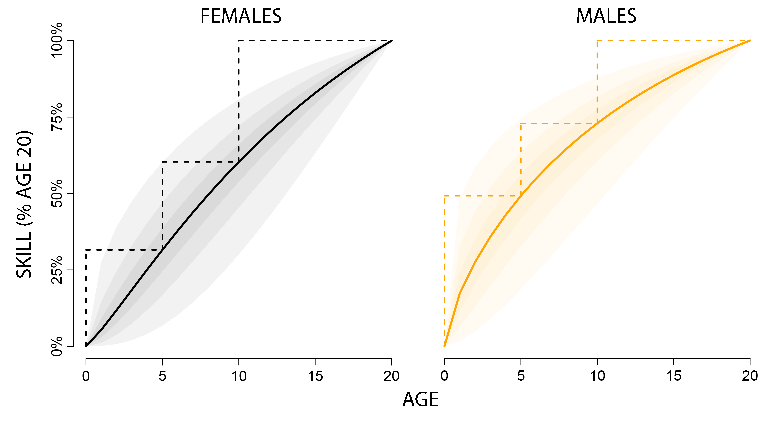
\includegraphics[width=12cm] {text/images/Figure_S2.pdf}
\renewcommand{\thefigure}{S\arabic{figure}}
\caption{\textbf{Predicted change in foraging skill by sex}. Values averaged over variation between studies, individuals, and resource type. The x-axis shows age, while the y-axis is an unit-free measure of the latent variable.}
\label{fig:sex_diffs}
\end{figure}


\begin{figure}[h]
\centering
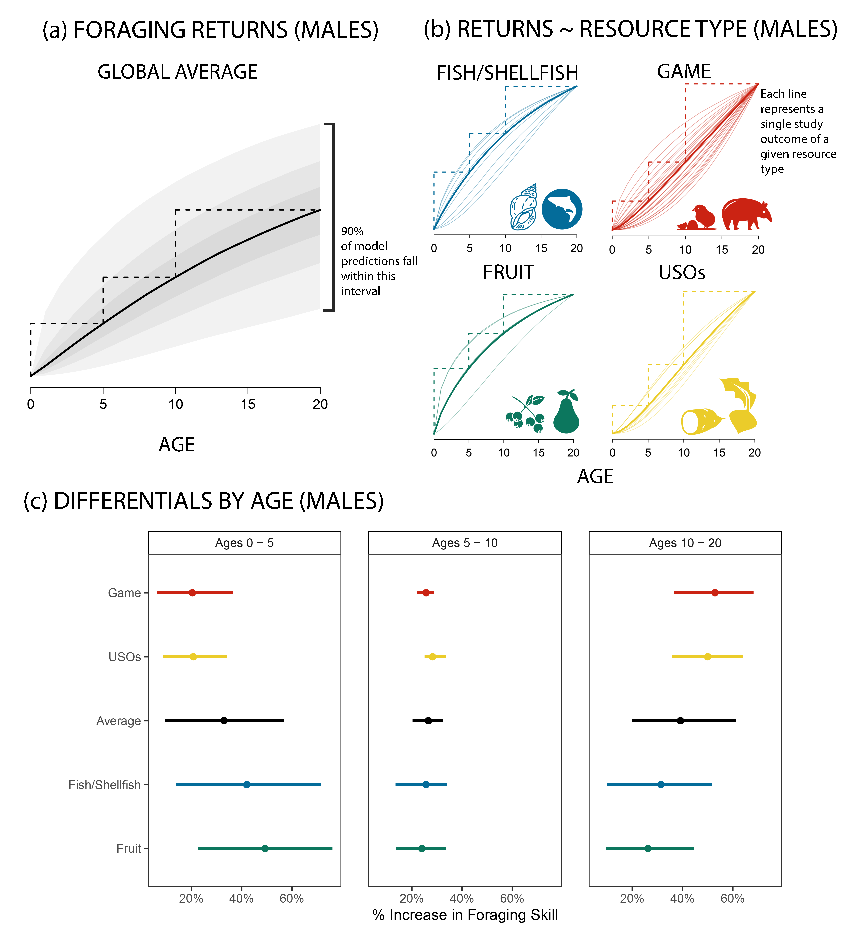
\includegraphics[width=12cm] {text/images/Figure_S3.pdf}
\renewcommand{\thefigure}{S\arabic{figure}}
\caption{\textbf{Foraging returns for females only.} (A)Predicted change in foraging returns with age, averaging over variation between studies, individuals, and resource type. The x-axis shows age, while the y-axis is an unit-free measure of the proportion of increase compared to the maximum value (predicted returns at age 20).} Solid line is the posterior median prediction, shaded intervals depict the 30th, 60th, and 90th percentile credible intervals. \textcolor{red}{Dashed lines highlight arbitrary age differentials across childhood. (B) Predicted change in foraging returns by resource type, with solid line denoting the average posterior median and transparent lines denoting the median for each unique study outcome for that resource type. All curves are scaled by their maximum value (predicted returns at age 20). However, the shape of the curves illustrates how productivity increases with age. (C) Percentage increase in foraging returns across childhood, covering the intervals denoted by the dashed lines in A-B. Points indicate posterior median, bars indicate 90\% HPDI. This figure is similar to figure \ref{fig:returns}, but focuses only on females.}
\label{fig:females_only}
\end{figure}

\begin{figure}[h]
\centering
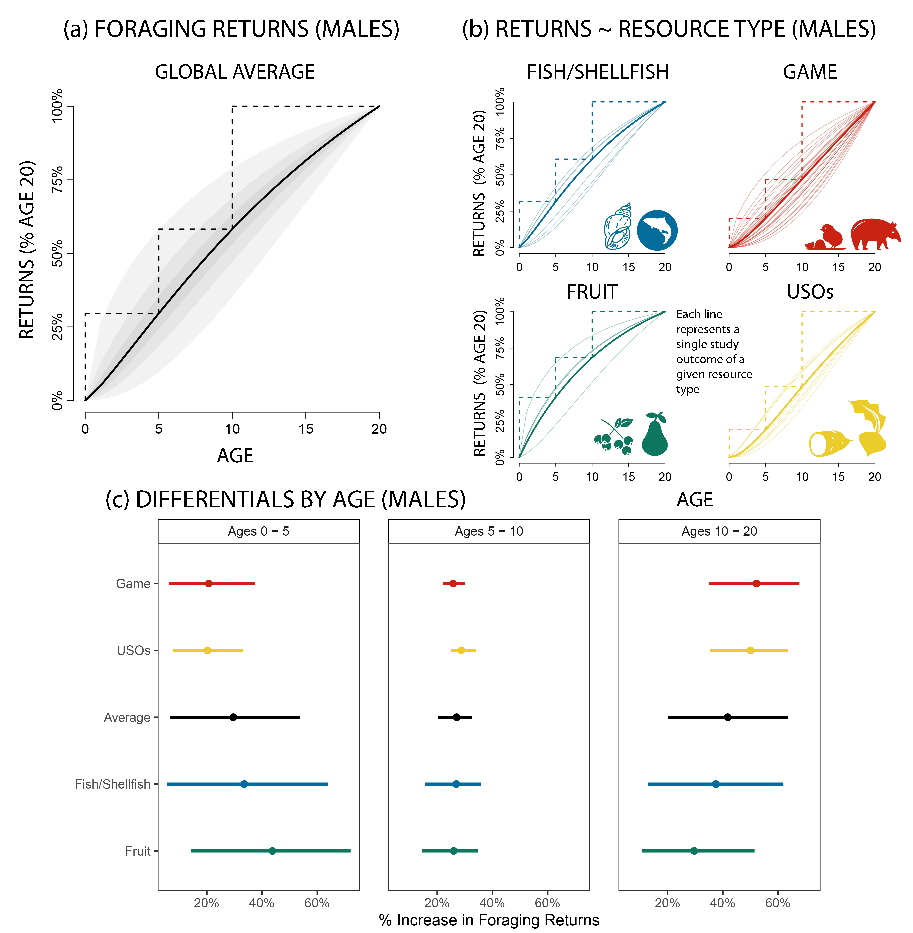
\includegraphics[width=12cm] {text/images/Figure_S4.pdf}
\renewcommand{\thefigure}{S\arabic{figure}}
\caption{\textbf{Foraging returns for males only.} (A)Predicted change in foraging returns with age, averaging over variation between studies, individuals, and resource type. \textcolor{red}{The x-axis shows age, while the y-axis is an unit-free measure of the proportion of increase compared to the maximum value (predicted returns at age 20).} Solid line is the posterior median prediction, shaded intervals depict the 30th, 60th, and 90th percentile credible intervals. \textcolor{red}{Dashed lines highlight arbitrary age differentials across childhood.} (B) Predicted change in foraging returns by resource type, with solid line denoting the average posterior median and transparent lines denoting the median for each unique study outcome for that resource type. All curves are scaled by their maximum value (predicted returns at age 20). However, the shape of the curves illustrates how productivity increases with age. (C) Percentage increase in foraging returns across childhood, covering the intervals denoted by the dashed lines in A-B. Points indicate posterior median, bars indicate 90\% HPDI. This figure is similar to figure \ref{fig:returns}, but focuses only on males.}
\label{fig:males_only}
\end{figure}

\begin{figure}[h]
\centering
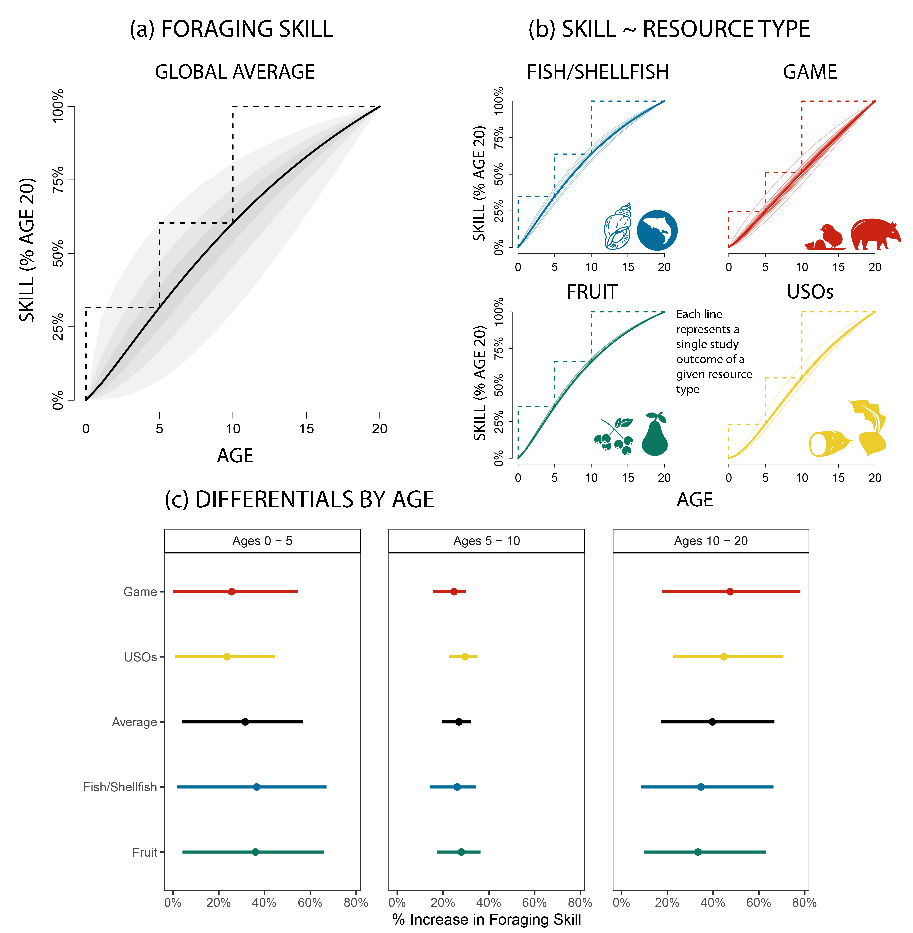
\includegraphics[width=12cm] {text/images/Figure_S5.pdf}
\renewcommand{\thefigure}{S\arabic{figure}}
\caption{\textbf{Foraging skill.} (A)Predicted change in foraging skill with age, averaging over variation between studies, individuals, sex, and resource type. \textcolor{red}{The x-axis shows age, while the y-axis is an unit-free measure of the proportion of increase compared to the maximum value (predicted returns at age 20).} Solid line is the posterior median prediction, shaded intervals depict the 30th, 60th, and 90th percentile credible intervals. \textcolor{red}{Dashed lines highlight arbitrary age differentials across childhood.} (B) Predicted change in foraging skill by resource type, with solid line denoting the average posterior median and transparent lines denoting the median for each unique study outcome for that resource type. All curves are scaled by their maximum value (predicted returns at age 20). However, the shape of the curves illustrates how skill increases with age. (C) Percentage increase in foraging skill across childhood, covering the intervals denoted by the dashed lines in A-B. Points indicate posterior median, bars indicate 90\% HPDI. This figure is similar to figure \ref{fig:returns}, but describe underlying foraging skill instead of returns.}
\label{fig:skill}
\end{figure}

\begin{figure}[h]
    \centering
    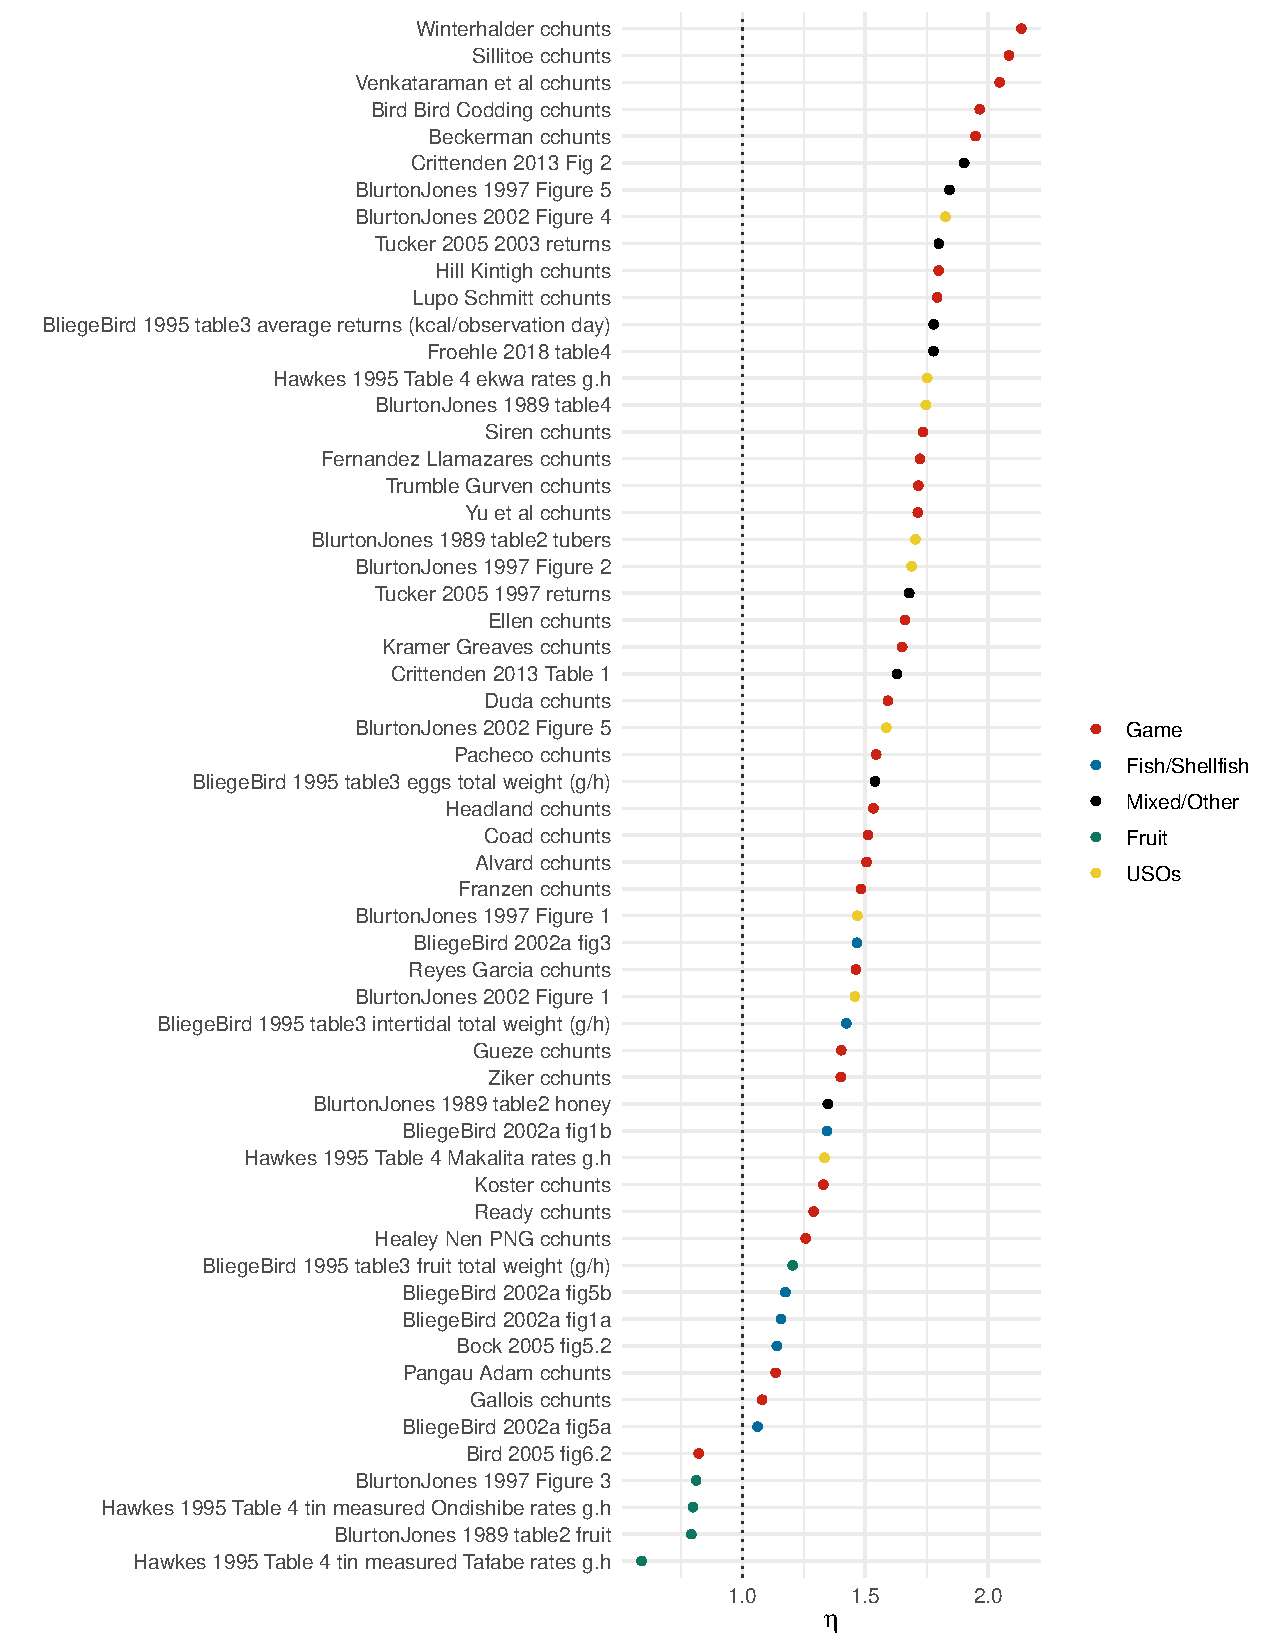
\includegraphics[width=12cm] {text/images/Figure_S6.pdf}
    \renewcommand{\thefigure}{S\arabic{figure}}
    \caption{\textbf{Mean skill intensity values.} Mean posterior values for $\eta$, the skill intensity of foraging, by outcome. Each individual dataset (either present in the \texttt{cchunts} package or extracted from a single figure/table) is represented here, color coded for resource. }
    \label{fig:eta_outcome}
\end{figure}
%bird 2005, which has lower eta, is the one where kids target age specific resources that have high returns. Might be an ecological outlier?

\begin{figure}
    \centering
    \renewcommand{\thefigure}{S\arabic{figure}}
    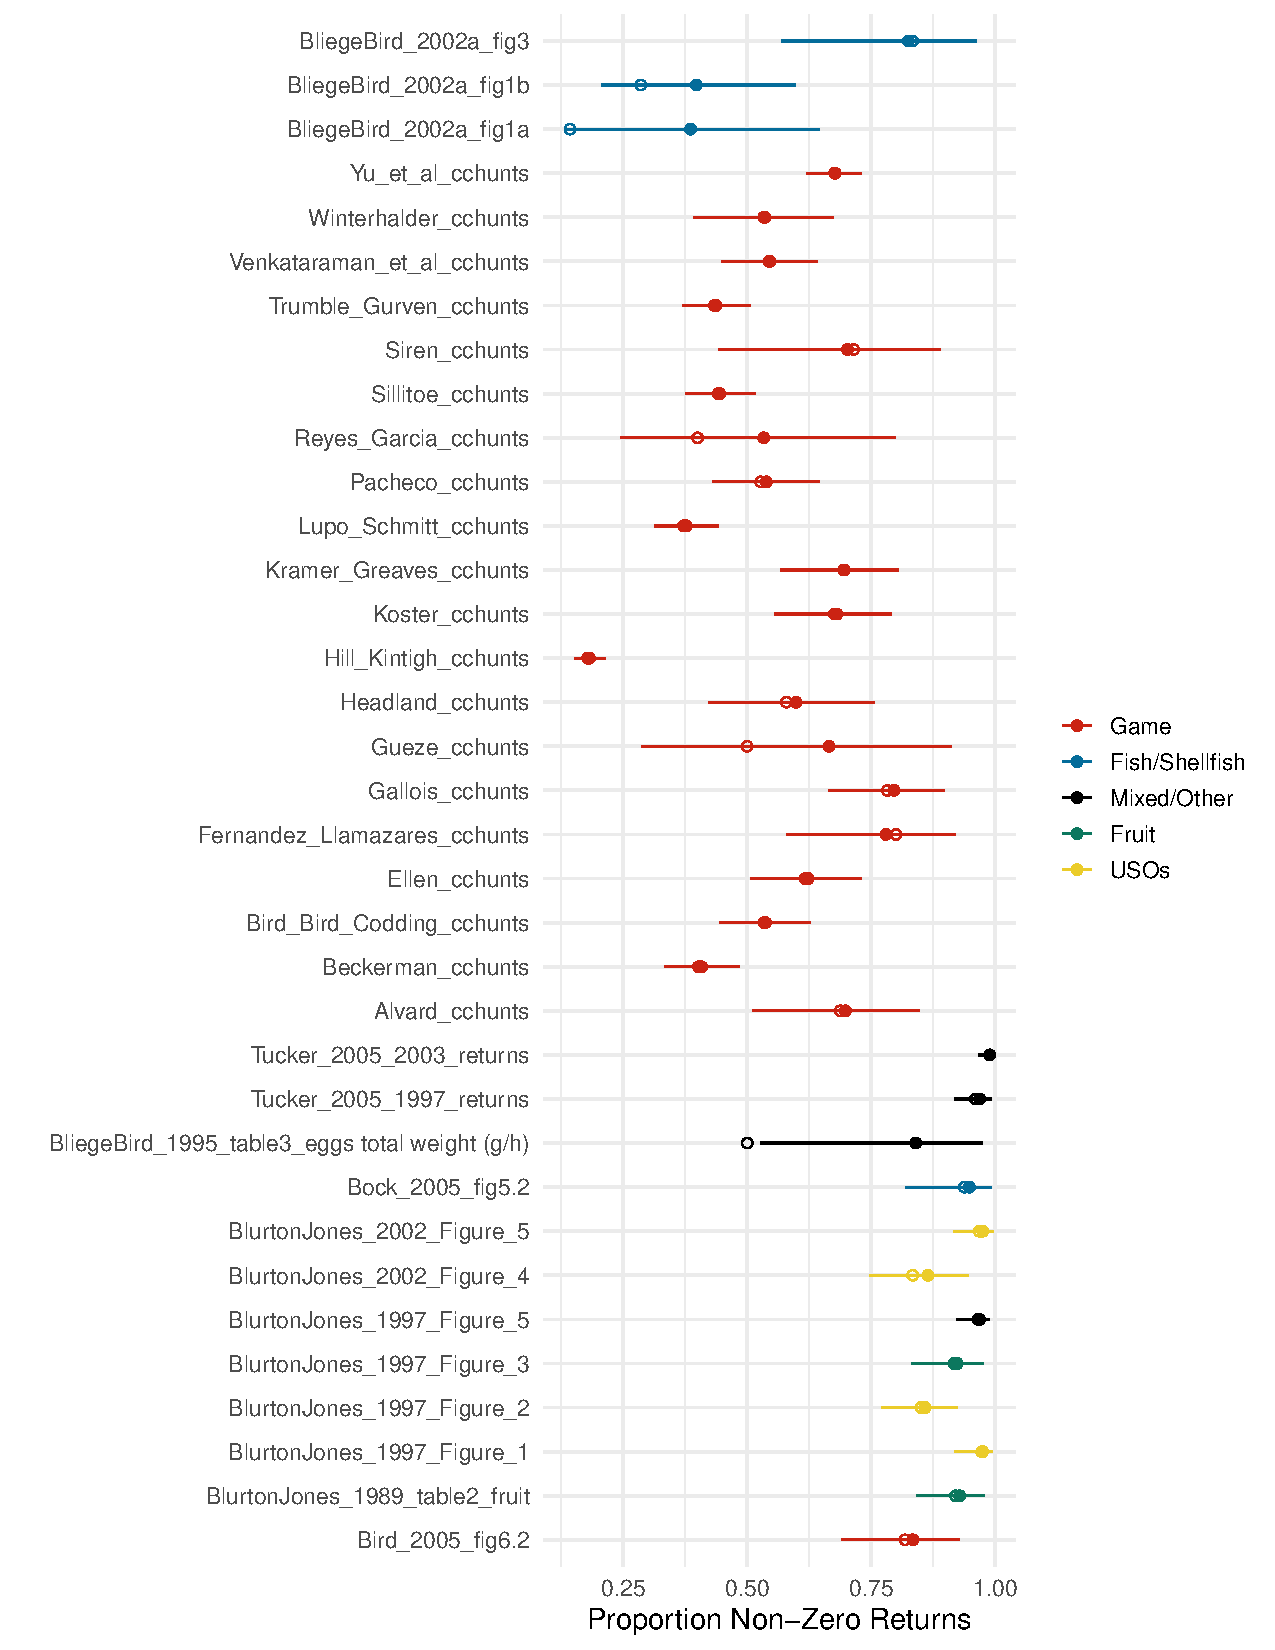
\includegraphics[width=12cm]{text/images/Figure_S7.pdf}
    \caption{\textbf{Real and estimated proportion non-zero returns by outcome.} Empty circles show real proportion of non-zero returns by outcome, mean and 95 percentile intervals of posterior distribution of estimated proportion of non-zero returns are indicated by full circles and bars. The model predicts with sufficient accuracy the proportion of non-zero returns.}
    \label{fig:non_zero}
\end{figure}

\begin{figure}[h]
\centering
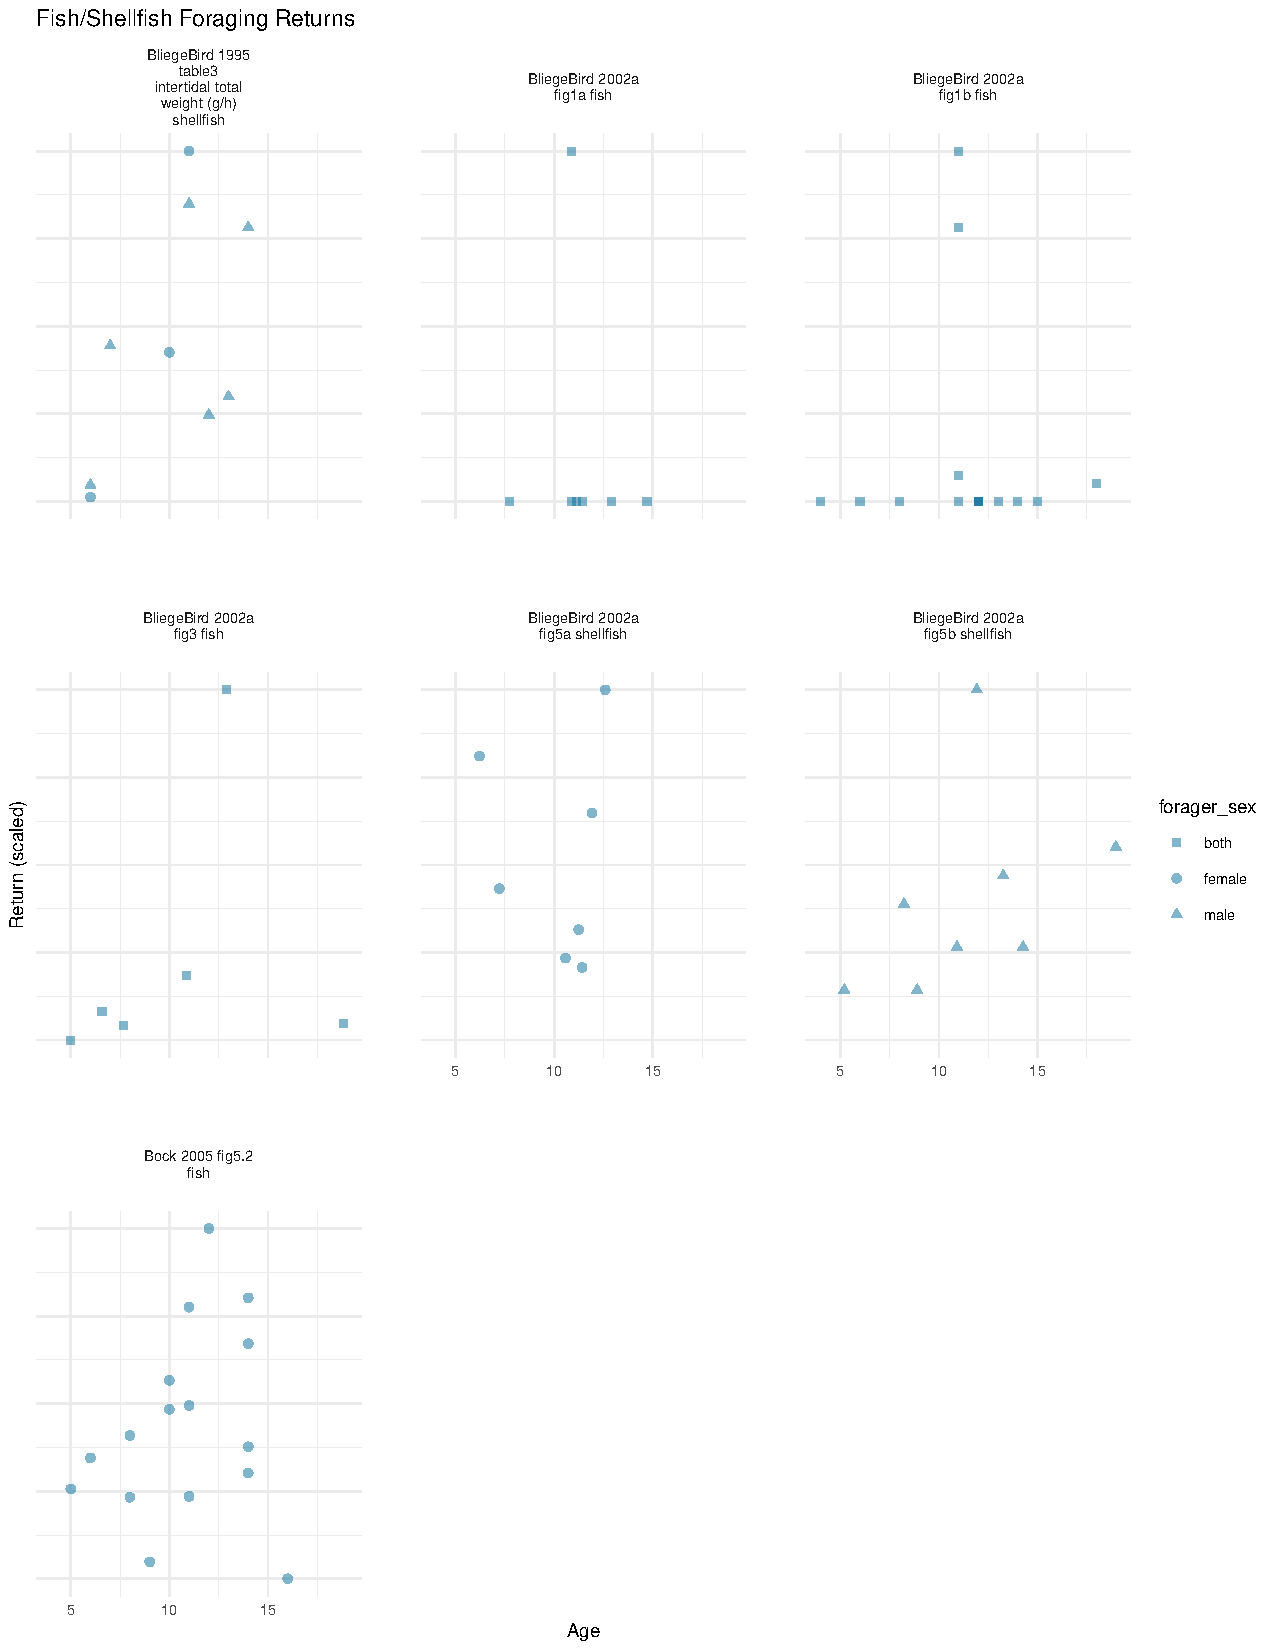
\includegraphics[width=12cm] {text/images/Figure_S8.pdf}
\renewcommand{\thefigure}{S\arabic{figure}}
\caption{\textbf{Fish data.} Data points for all datasets reporting fish and shellfish data.}
\label{fig:fish}
\end{figure}

\begin{figure}[h]
\centering
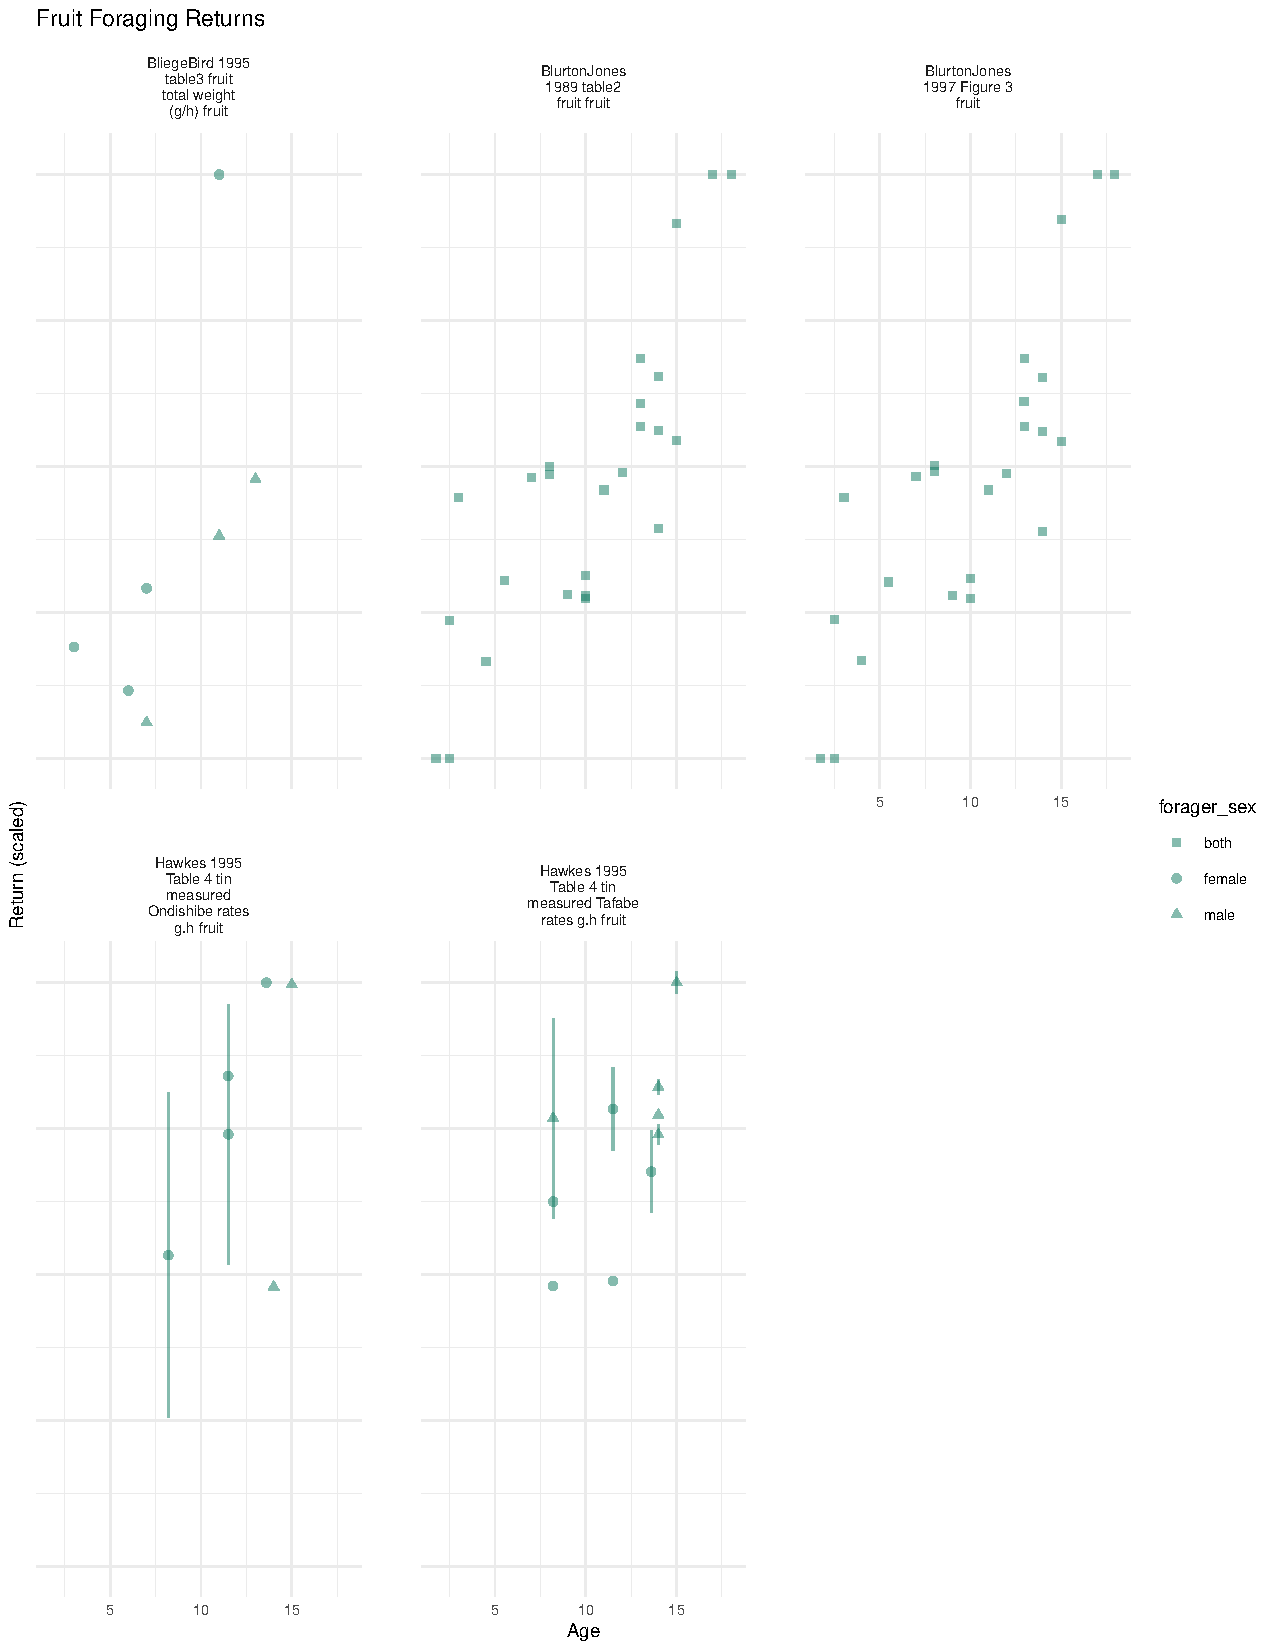
\includegraphics[width=12cm] {text/images/Figure_S9.pdf}
\renewcommand{\thefigure}{S\arabic{figure}}
\caption{\textbf{Fruit data.} Data points for all datasets reporting fruit data.}
\label{fig:fruit}
\end{figure}

\begin{figure}[h]
\centering
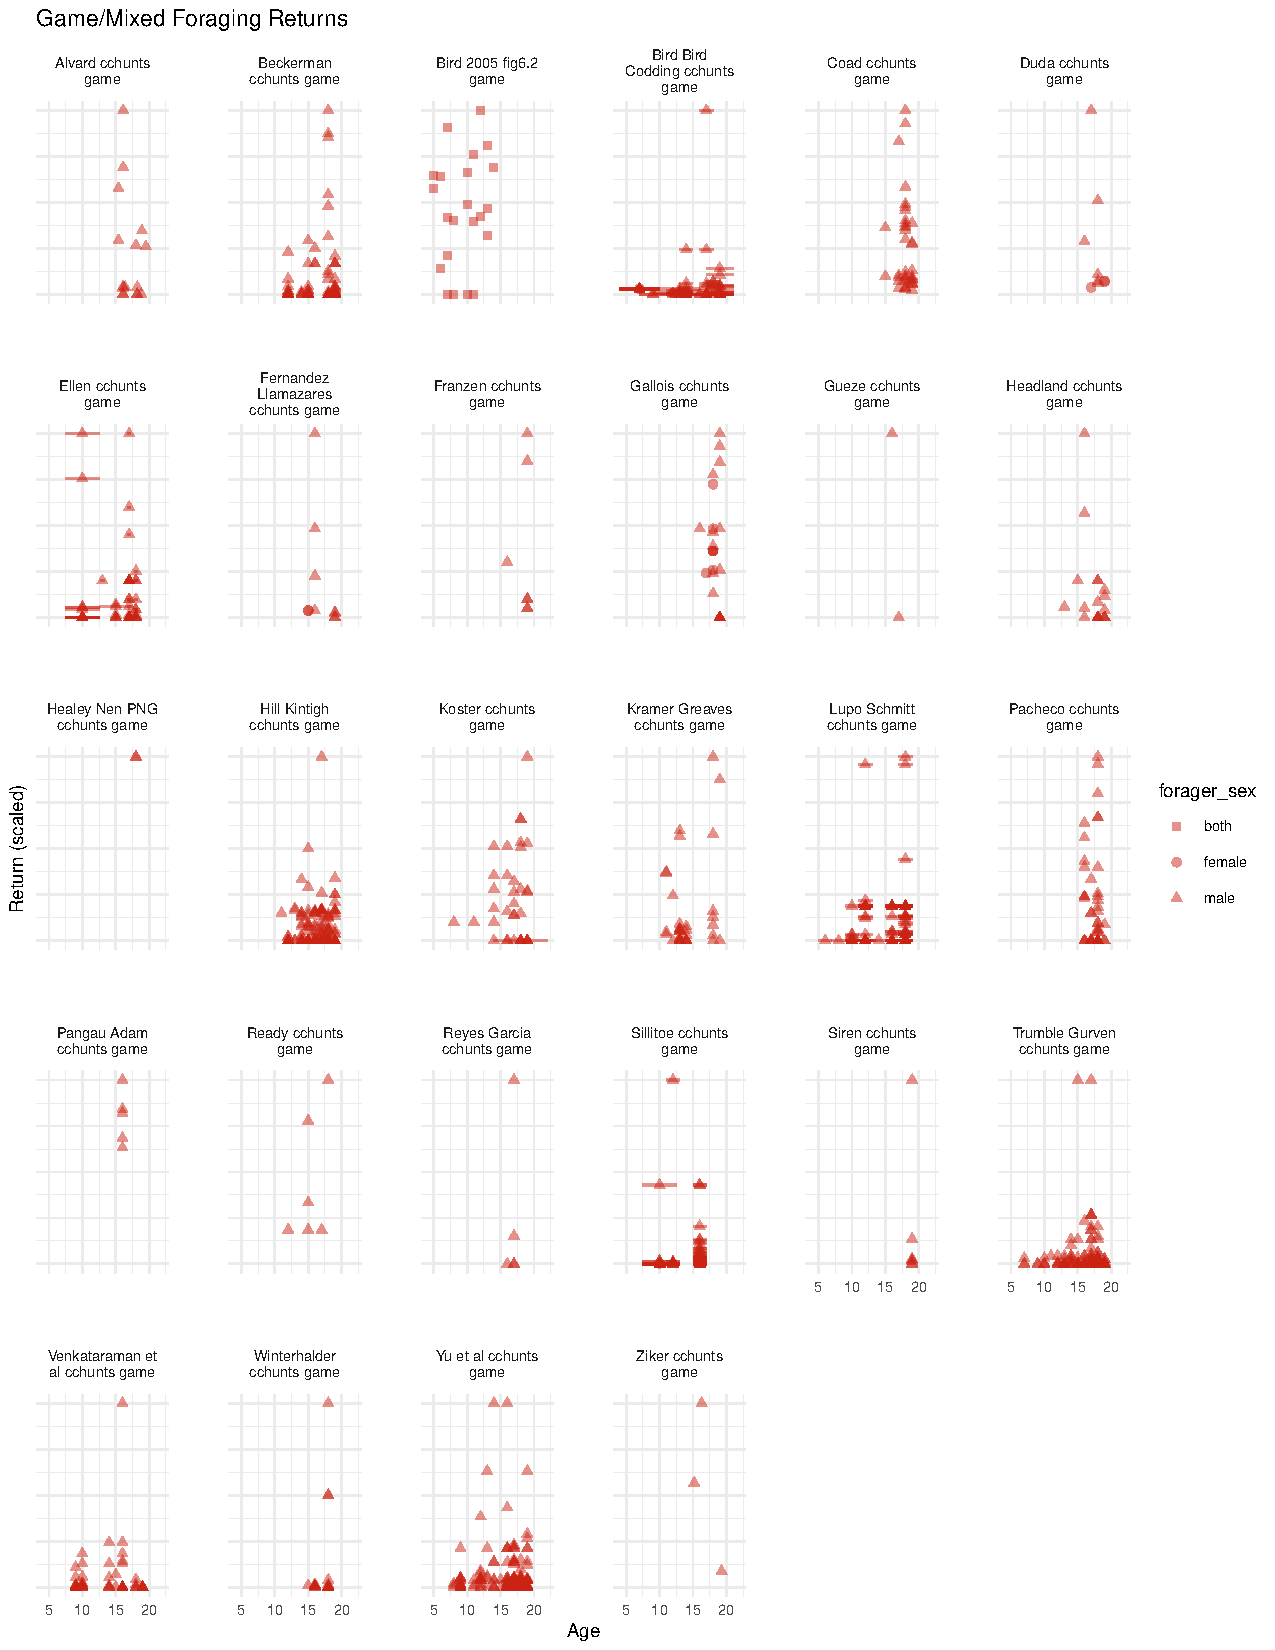
\includegraphics[width=12cm] {text/images/Figure_S10.pdf}
\renewcommand{\thefigure}{S\arabic{figure}}
\caption{\textbf{Game data.} Data points for all datasets reporting game data.}
\label{fig:game}
\end{figure}

\begin{figure}[h]
\centering
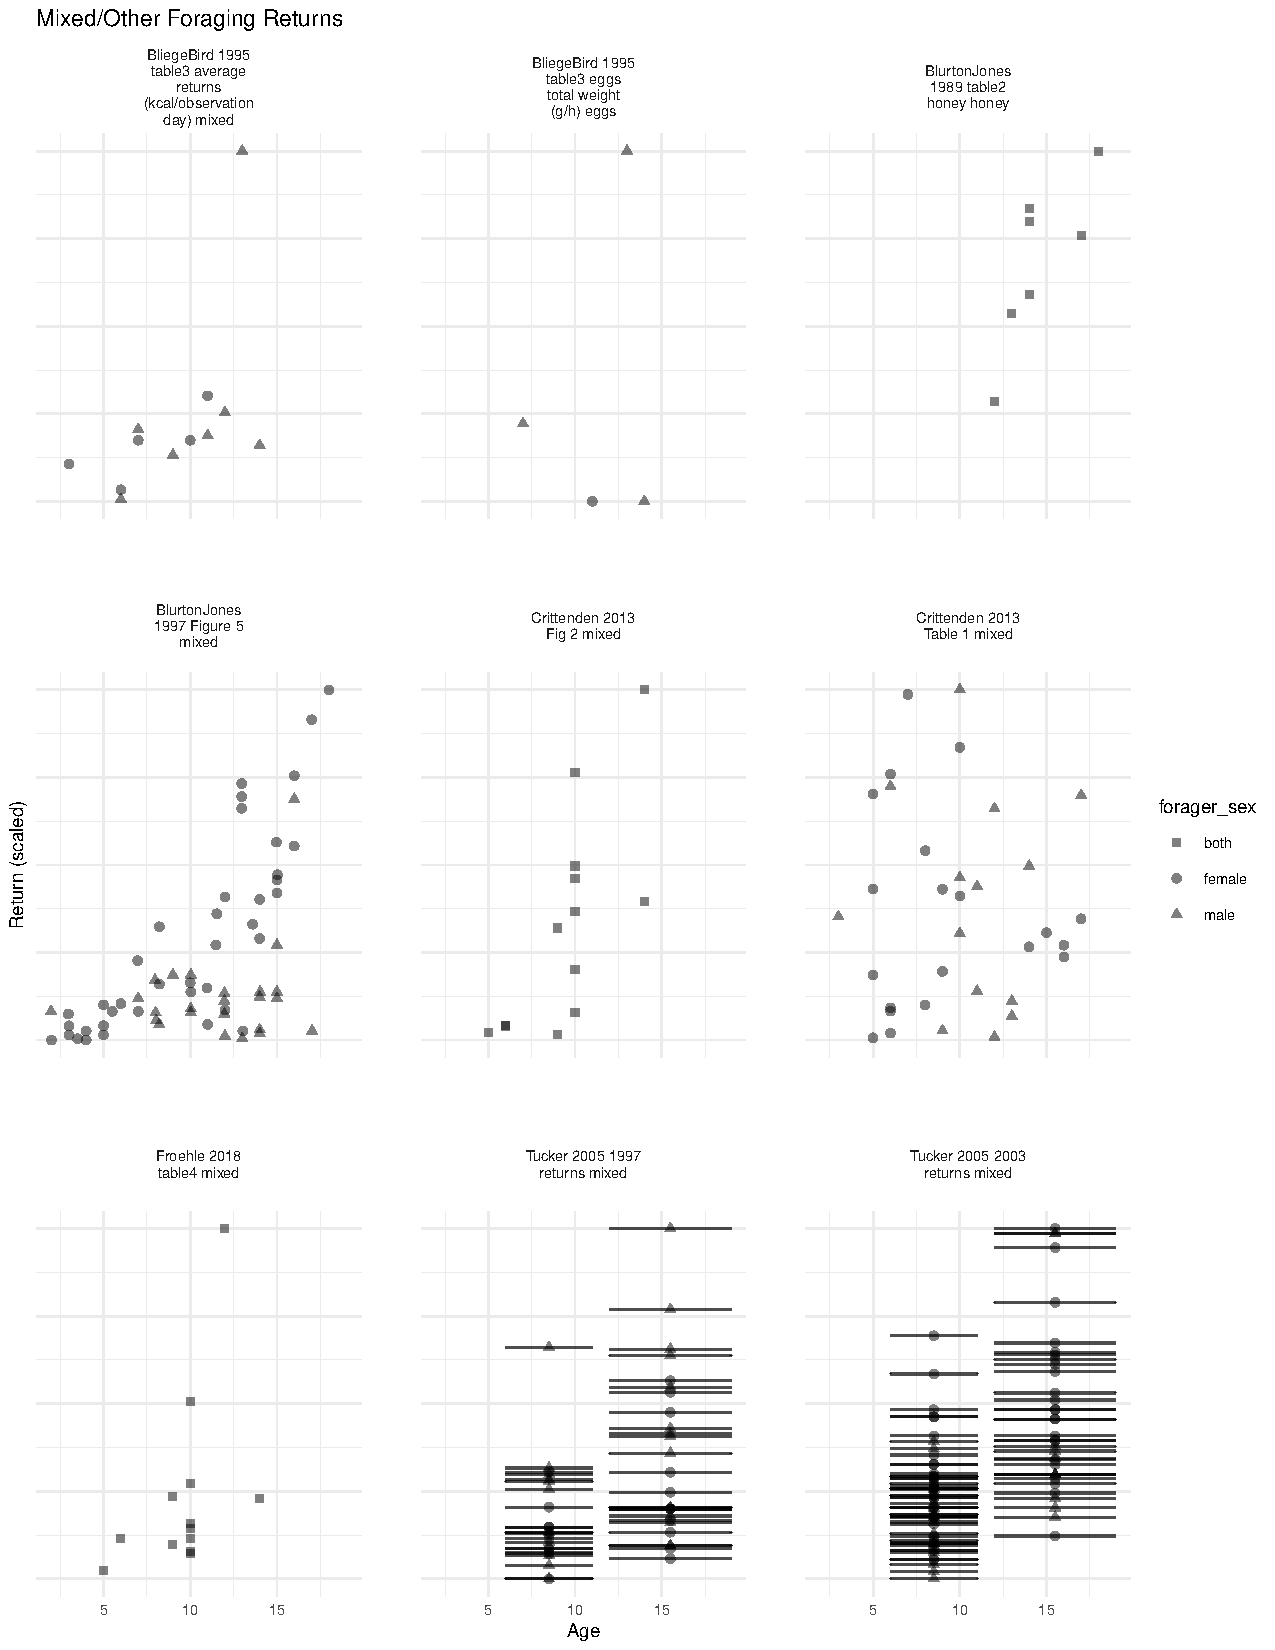
\includegraphics[width=12cm] {text/images/Figure_S11.pdf}
\renewcommand{\thefigure}{S\arabic{figure}}
\caption{\textbf{Data from other resources.} Data points for all datasets reporting data for other kinds of resources.}
\label{fig:other}
\end{figure}

\begin{figure}[h]
\centering
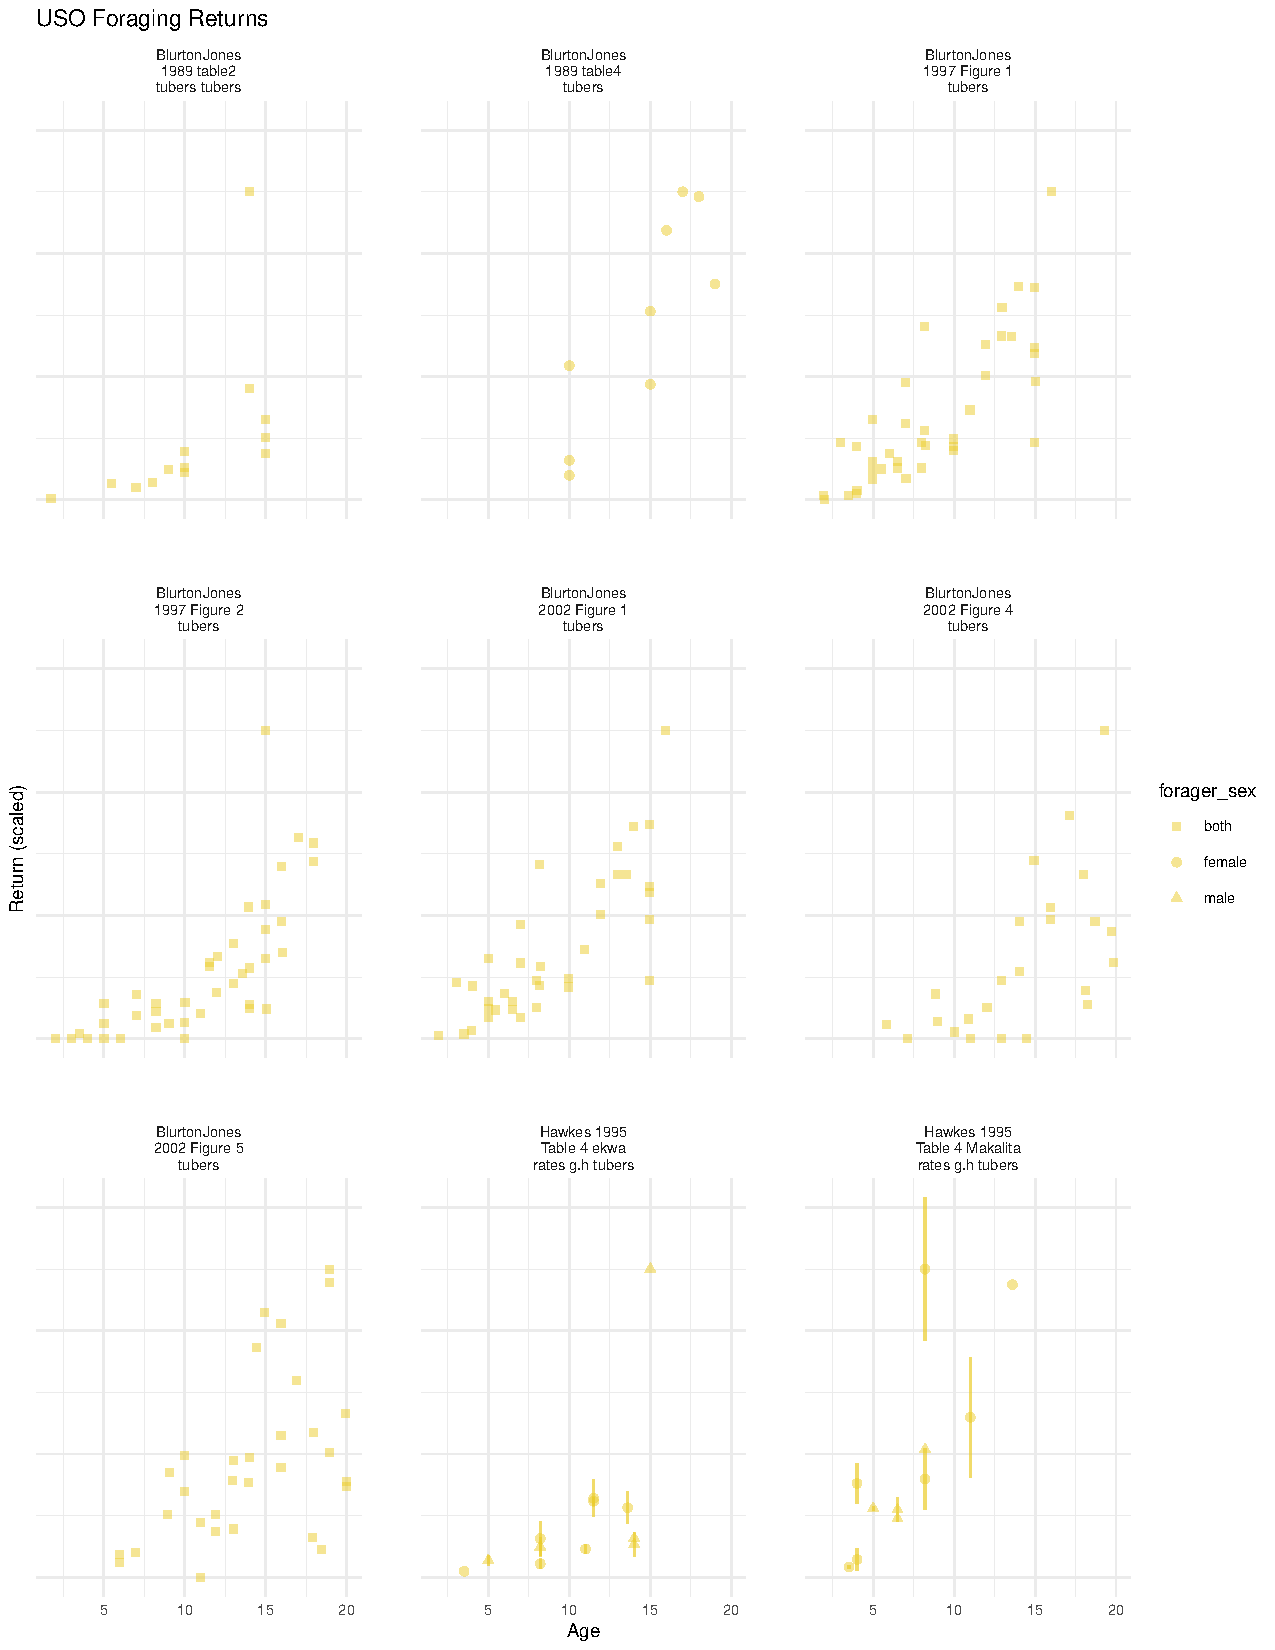
\includegraphics[width=12cm] {text/images/Figure_S12.pdf}
\renewcommand{\thefigure}{S\arabic{figure}}
\caption{\textbf{Tubers data.} Data points for all datasets reporting tuber data.}
\label{fig:USO}
\end{figure}